\chapter{波动光学}
\section{光波;光屏上的波函数}
在波动光学中,几束光射到同一个地方,光强不是简单的相加,而是光波的叠加,可能增强也可能减弱。(这一章里光强指的是能量通量密度,也就是单位时间、单位面积通过的能量,而眼睛感受到的光强测量起来更加复杂)

三维空间中的一个光源发出球面电磁波,波函数$\psi(r,t)=\frac{A_0}{r} \rme^{\rmi(k r-\omega t)}$,电磁场的每个分量都可以这样表示。(啊。。这不是量子力学里的波函数,如果是机械波的话$\psi$就是某个点在某个时刻的位移,电磁波的话就叫波函数好了)

跟前面一样,为了加减的运算方便,把它表示成复指数,但是乘除之前要先取实部。$\frac{A_0}{r}$是与光源距离为$r$的某个点上波的振幅,$\rme^{\rmi(k r-\omega t)}$则是相位。$A_0$表示光源的强度,同一个光源的$A_0$是相同的,这一章里先不管它。而且只考虑同一时刻的波,因此也不管$\rme^{-\rmi \omega t}$。$k=\frac{2 \pi}{\lambda}$,$\lambda$是波长。在同一时刻,距离每增加$\lambda$,相位就增加$2 \pi$。

振幅与$r$成反比,而光强是振幅的平方,与$r^2$成反比,这样才能保证任何一个球面上的能量通量$\Phi=(\frac{A_0}{r})^2 \cdot 4 \pi r^2$与$r$无关,能量是守恒的。

如图\ref{fig-wave-amp},在空间中有一个光屏和主光轴,交点为$O$。光源$S$在主光轴上,到光屏的距离为$z$,光屏上一点$P$到$O$的距离为$x$(以后还会把光屏看作$x-y$平面),那么$r=\sqrt{z^2+x^2}$。
\begin{figure}[htb]
\centering
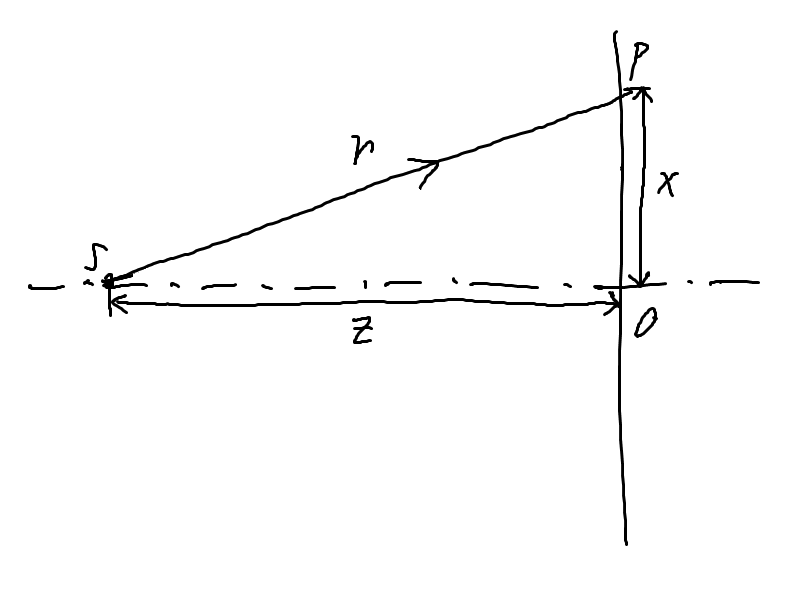
\includegraphics[scale=0.5]{fig/wave-amp.png}
\caption{传说主光轴要画成点划线但是手画很麻烦}
\label{fig-wave-amp}
\end{figure}

接下来要做一个近似:当$x \ll z$时,$r=z (1+\frac{x^2}{2 z^2})$,这个条件称为傍轴条件,因为光射到的位置离主光轴很近。这时振幅$\frac{A_0}{r}=\frac{A_0}{z (1+\frac{x^2}{2 z^2})}=\frac{A_0}{z}(1-\frac{x^2}{2 z^2})$,忽略高阶项,就是$\frac{A_0}{z}$。

而相位$\rme^{\rmi k r}=\rme^{\rmi k z} \rme^{\rmi k \frac{x^2}{2 z}}$。第一项$\rme^{\rmi k z}$与$x$无关,可以并到振幅里面去。然而$\lambda$很小,$k$很大,即使$x$有一点点变化,第二项$\rme^{\rmi k \frac{x^2}{2 z}}$也有很大的变化,不能再对它做近似。

(非要作近似也可以,当$\frac{x^2}{\lambda z} \ll 1$时,球面波就被近似成了平面波,整个光屏上的相位是一样的。这种情况称为远场条件)

如果光源不在主光轴上,到主光轴的距离为$x_0$(在同一个平面上),可以把$x$改成$x-x_0$。最后光屏上的波函数是
\begin{equation*}
\psi(x,x_0)=A \rme^{\rmi k \frac{(x-x_0)^2}{2 z}}
\end{equation*}

如果有几束光射到同一个地方,它们的波函数可以相加,光强则是波函数之和的模长的平方,跟量子力学当中波函数与概率的关系差不多。

(要求这几束光是相干的,也就是它们的振动方式一样,这又是一个复杂的问题。现在我们只要知道,同一个光源发出的光是相干的,被双缝分成两份之后也是)
\section{双缝干涉}
高中物理课本讲过双缝干涉,可以用小角近似的方法算条纹间距(虽然有些版本的课本连公式都没有讲)。这里用波函数的方法再算一遍。

设两条缝在$\pm x_0$处,光屏上的波函数$\psi=A (\rme^{\rmi k \frac{(x-x_0)^2}{2 z}}+\rme^{\rmi k \frac{(x+x_0)^2}{2 z}})$,光强则是
\begin{align*}
F&=\psi \psi^* \\
&=A^2 (\rme^{\rmi k \frac{(x-x_0)^2}{2 z}}+\rme^{\rmi k \frac{(x+x_0)^2}{2 z}})(\rme^{-\rmi k \frac{(x-x_0)^2}{2 z}}+\rme^{-\rmi k \frac{(x+x_0)^2}{2 z}}) \\
&=A^2 (2+\rme^{\rmi k B}+\rme^{-\rmi k B}) \\
&=A^2 (2+2 \cos k B) \\
&=4 A^2 \cos^2 \frac{k B}{2} \\
\text{其中}B&=\frac{(x+x_0)^2-(x-x_0)^2}{2 z} \\
&=\frac{2 x_0 x}{z} \\
F&=4 A^2 \cos^2 \frac{k x_0}{z} x \\
&=4 A^2 \cos^2 2 \pi \frac{x_0}{\lambda z} x
\end{align*}

所以光强$F$是余弦的平方,周期为$\frac{\lambda z}{2 x_0}$。而双缝的间距$d=2 x_0$,所以周期为$\frac{\lambda z}{d}$。不但能算出两个最亮处或者最暗处的间距,还能算出其他地方的光强。

要强调的是,这些结果只有在傍轴近似下成立,所以只有双缝正对着的一小块地方能看到清晰的条纹,我们平常看到一大排条纹的图片一般是放大过的。
\section{无穷远处的波函数}
距离为$z$的光屏上有波函数,无穷远处也有波函数。如图\ref{fig-wave-amp-inf}左侧,光源是一个一维的物体,有一根主光轴与它垂直,交点$S$的坐标为$0$。物体向无穷远处的各个方向射出平行光(图中只画了一个方向),与主光轴的夹角为$\theta$。这一章里$\theta \ll 1$。
\begin{figure}[htb]
\centering
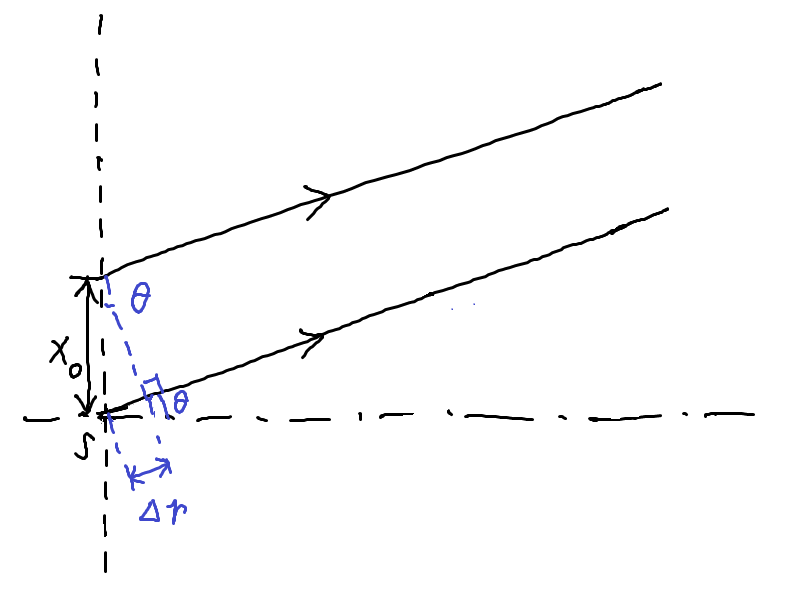
\includegraphics[scale=0.5]{fig/wave-amp-inf.png}
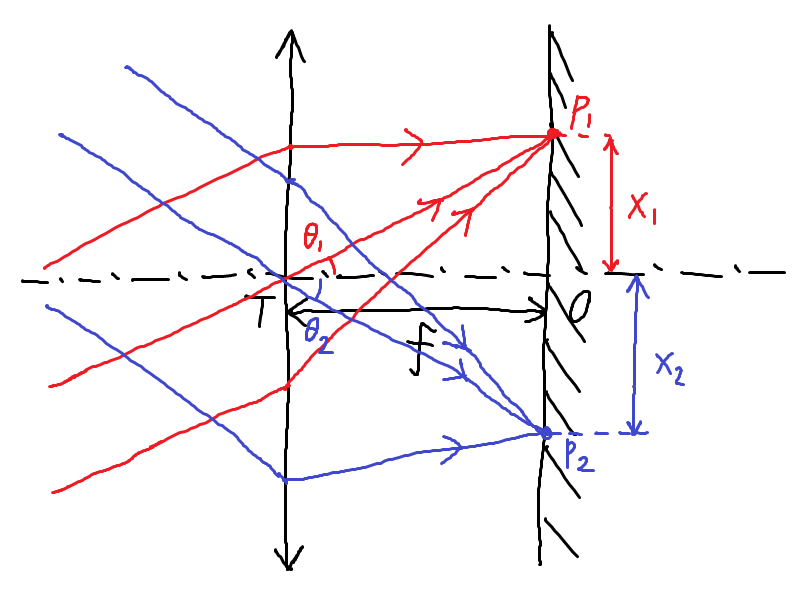
\includegraphics[scale=0.5]{fig/conv-lens.png}
\caption{射向无穷远,再用凸透镜聚焦}
\label{fig-wave-amp-inf}
\end{figure}

(注意这里的所有结论都在$\theta \ll 1$时才成立,图中为了清楚把$\theta$画得比较大)

物体上可以有很多个点发光,如果一个点与$S$的距离为$x_0$,它发出的光比$S$处的光少走光程$\delta r=x_0 \sin \theta=x_0 \theta$,相位差为$\rme^{-\rmi k x_0 \theta}$。

用凸透镜可以把一束射向无穷远的平行光聚焦到一个点上。如图\ref{fig-wave-amp-inf}右侧,角度为$\theta$的平行光聚焦到点$P$,位置$x=f \sin \theta=f \theta$,$f$是透镜的焦距。把射到$P$点的每条光线的波函数加起来,就是$P$点上的波函数,也代表无穷远处$\theta$方向的波函数。

(这里的平行光是无限宽的,透镜也是无限大的,所以上下移动平行光不会改变聚焦的位置,只有改变平行光的方向才能改变聚焦的位置。无限宽的平行光和傍轴近似是矛盾的,但是这里就这么算吧,反正是理想模型。另外,每条光线通过透镜的光程都是相同的,这个问题也不讲了)

高中做双缝干涉的实验时一般不会在屏前面用凸透镜成像。如果用凸透镜成像,观察无穷远处的光强,结果会怎么样呢?
\begin{align*}
\psi&=A(\rme^{-\rmi k x_0 \theta}+\rme^{\rmi k x_0 \theta}) \\
&=2 A \cos k x_0 \theta \\
F&=\psi \psi^* \\
&=4 A^2 \cos^2 k x_0 \theta \\
&=4 A^2 \cos^2 \frac{k x_0}{z} x \\
&=4 A^2 \cos^2 2 \pi \frac{x_0}{\lambda z} x
\end{align*}

在我们的近似下,结果和有限远处一样,但是计算会简便一些。接下来的问题严格来说都要用凸透镜来聚焦平行光,但是实验当中经常会直接用屏来成像,只要屏够远,误差不会很大。
\section{单缝衍射}
如图\ref{fig-silt-diff},一条狭缝宽度为$a$,里面的每个点都射出光线。我们一般把有限个光源的叠加叫干涉,而把无限个光源的叠加叫衍射。
\begin{figure}[htb]
\centering
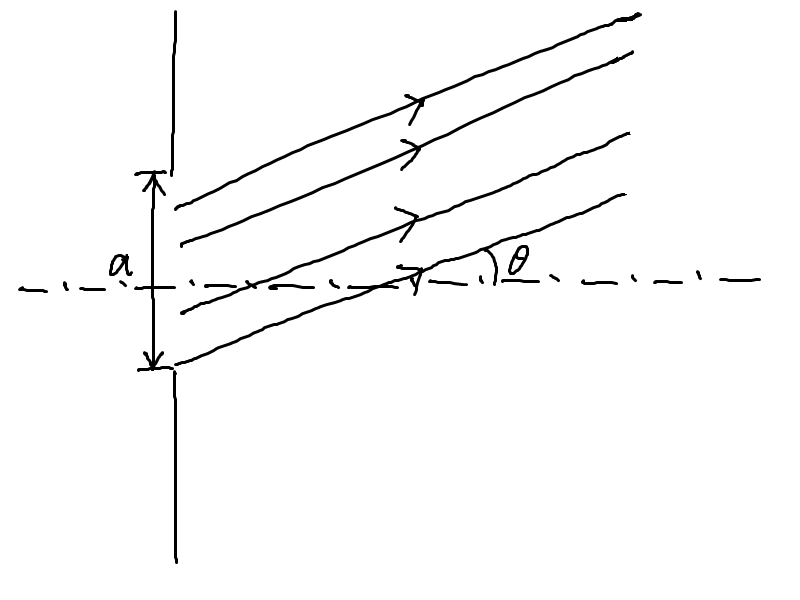
\includegraphics[scale=0.5]{fig/silt-diff.png}
\caption{这条缝其实是很细的}
\label{fig-silt-diff}
\end{figure}

计算波函数需要积分:
\begin{align*}
\psi&=\int_{-\frac{a}{2}}^{\frac{a}{2}} A \rme^{-\rmi k x_0 \theta} \opd x_0 \\
&=\frac{\rmi A}{k} (\rme^{-\rmi \frac{k a \theta}{2}}-\rme^{\rmi \frac{k a \theta}{2}}) \\
&=2 \frac{A}{k} \sin \frac{k a \theta}{2}
\end{align*}

设$\alpha=\frac{k a \theta}{2}=\frac{\pi a \theta}{\lambda}$,那么$\psi=A \frac{\sin \alpha}{\alpha}$。$\frac{\sin x}{x}$是一个在光学中经常用到的函数,有些地方叫作\emph{读数函数}或者$\sinc x$。

光强则是$F=\psi^2=A^2 (\frac{\sin \alpha}{\alpha})^2$,如图\ref{fig-silt-diff-plot},中间有一个明显的峰,称为零级峰,旁边还有一级峰,二级峰等等,但是在实验中不容易看到。从图像下面的面积可以看出,零级峰占了总能量的90\%。
\begin{figure}[htb]
\centering
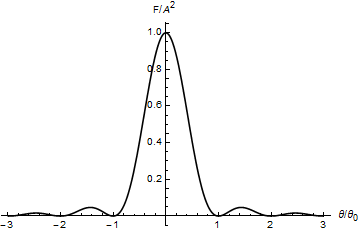
\includegraphics[scale=0.5]{fig/silt-diff-plot.png}
\caption{迷之凸起}
\label{fig-silt-diff-plot}
\end{figure}

$\alpha$是一个无量纲的数。$\theta=\frac{\lambda}{a}$时,$\alpha=\pi$,$F=0$,所以它是零级峰的半角宽度。注意它是一个角度,零级峰的宽度还要取决于聚焦用的透镜焦距。增大$\lambda$或者减小$a$,条纹就会变宽。

一般认为缝宽$a$是光波长$\lambda$的$\frac{1}{5}$到$5$倍时,衍射是比较明显的。可见光的波长是几百纳米,而实验用的缝宽一般是几微米。
\section{双缝干涉中的衍射}
刚才把双缝干涉的每条缝都当作一个点,实际上它们发出的光也会衍射,有什么影响呢?

一条缝发出的波函数就是$\psi_1=A \frac{\sin \alpha}{\alpha}$,另一条缝与它的距离是$d$,可以直接乘上一个相位差$\rme^{-\rmi k d \theta}$。两条缝的波函数之和是
\begin{align*}
\psi&=\psi_1 (1+\rme^{-\rmi k d \theta}) \\
&=2 \psi_1 \cos \frac{k d \theta}{2} \rme^{-\rmi \frac{k d \theta}{2}} \\
&=2 \rme^{-\rmi \frac{k d \theta}{2}} A \frac{\sin \alpha}{\alpha} \cos \frac{k d \theta}{2}
\end{align*}

$2 \rme^{-\rmi \frac{k d \theta}{2}} A$是常数,这里不用考虑。设$\beta=\frac{k d \theta}{2}$,那么$F=\psi^2=(\frac{\sin \alpha}{\alpha} \cos  \beta)^2$,也就是双缝干涉的光强乘上了一个单缝衍射的光强。

$\frac{d}{a}=10$时,$F$的图像如图\ref{fig-silt-diff-plot-2}。双缝干涉会产生比较密的峰$(\cos \beta)^2$,而单缝衍射的因子$(\frac{\sin \alpha}{\alpha})^2$让远处的峰高度降低。
\begin{figure}[htb]
\centering
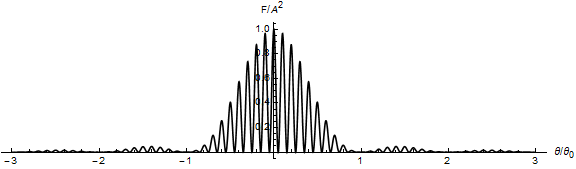
\includegraphics[scale=0.5]{fig/silt-diff-plot-2.png}
\caption{峰里有峰}
\label{fig-silt-diff-plot-2}
\end{figure}

为了清楚,画图时的$\frac{d}{a}$比较小。实验中$a$一般是几微米,而$d$是几毫米,$\frac{d}{a}=1000$,单缝衍射的零级峰里可以放下更多双缝干涉的峰。再加上小角近似的限制,实验中观察到的干涉条纹只有最中间那几条,而缝宽对它们几乎没有影响。
\section{形状因子与结构因子}
现在双缝干涉的波函数可以分成两部分:形状因子$\psi_f=\frac{\sin \alpha}{\alpha}$表示每根缝的形状,结构因子$\psi_s=\cos \beta$表示两根缝的位置关系,而$\psi=\psi_f \psi_s$。如果把两根缝换成圆孔或者其他东西,只要改变$\psi_f$;如果增加更多的缝,或者改变缝的相对位置和相对光强,只要改变$\psi_s$。

举个栗子:如果有三根缝分别在位置$0,x_1,x_2$,相对光强分别为$1,2,3$,可以直接写出$\psi=\frac{\sin \alpha}{\alpha}(1+2 \rme^{-\rmi k x_1 \theta}+3 \rme^{-\rmi k x_2 \theta})$,形状因子还是单缝,结构因子则是$\psi_s=1+2 \rme^{-\rmi k x_1 \theta}+3 \rme^{-\rmi k x_2 \theta}$。

我们知道X射线衍射可以分辨晶体的结构,而晶体是由许多相同的分子排列成的,衍射图案可以反映出分子形状和排列方式,把衍射图案分成形状因子与结构因子就是把两者分开。
\section{光栅}
把许多狭缝排在一起就变成了光栅(读作shān)。设光栅上总共有$N$条缝,每条缝的宽度为$a$,缝与缝之间不透光部分的宽度为$b$。如果把一条缝平移$d=a+b$,就与另一条缝重合,所以我们用$d$表示缝的距离(而不是$b$)。一般的光栅每毫米有几百条缝。

光栅的形状因子仍然是$\frac{\sin \alpha}{\alpha}$,而结构因子是等比数列:
\begin{align*}
\psi_s&=1+\rme^{-\rmi k d \theta}+\rme^{-2 \rmi k d \theta}+\dots+\rme^{-(N-1) \rmi k d \theta} \\
&=\frac{1-\rme^{-\rmi N k d \theta}}{1-\rme^{-\rmi k d \theta}} \\
&=\frac{\rme^{-\rmi N \frac{k d \theta}{2}} (\rme^{\rmi N \frac{k d \theta}{2}}-\rme^{-\rmi N \frac{k d \theta}{2}})}{\rme^{-\rmi \frac{k d \theta}{2}} (\rme^{\rmi \frac{k d \theta}{2}}-\rme^{-\rmi \frac{k d \theta}{2}})} \\
&=\rme^{-\rmi (N-1) \frac{k d \theta}{2}} \frac{\sin N \beta}{\sin \beta}
\end{align*}

其中$\beta$仍然是$\frac{k d \theta}{2}$。$N=2$时,就是上面的双缝干涉。

光强$F=\psi \psi^*=(\frac{\sin \alpha}{\alpha})^2 (\frac{\sin N \beta}{\sin \beta})^2$。$\frac{d}{a}=10,N=2,4,6,8$时,$F$如图\ref{fig-grate}。可以看出,$N$越大,条纹越尖锐。
\begin{figure}[htb]
\centering
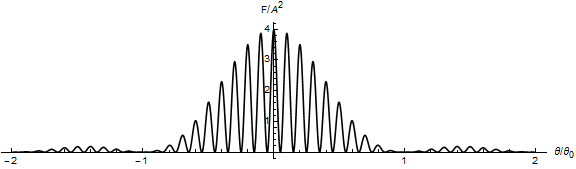
\includegraphics[scale=0.3]{fig/grate-2.png}
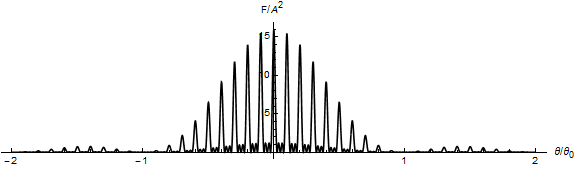
\includegraphics[scale=0.3]{fig/grate-4.png} \\
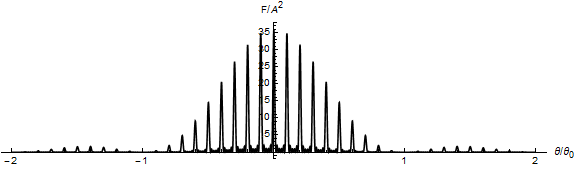
\includegraphics[scale=0.3]{fig/grate-6.png}
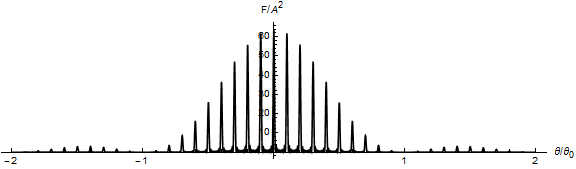
\includegraphics[scale=0.3]{fig/grate-8.png}
\caption{如果$N$和$\frac{d}{a}$很大的话图片根本看不清}
\label{fig-grate}
\end{figure}
\section{衍射与傅立叶变换}
(这一节也要看过后面的傅立叶变换才能看)

一个一维的物体可以看成亮度关于位置的函数$A(x_0)$。它可以有些地方发光,有些地方不发光,发光的地方亮度也可以不一样。无穷远处的波函数可以表示成积分:
\begin{equation*}
\psi(\theta)=\int_{-\infty}^{\infty} A(x_0) \rme^{-\rmi k x_0 \theta} \opd x_0
\end{equation*}

而傅立叶变换的公式是:
\begin{align*}
g(k)&=\mathscr{F}_{x \rightarrow k} f(x)=\frac{1}{\sqrt{2 \pi}} \int_{-\infty}^{\infty} f(x) \rme^{-\rmi k x} \opd x &
f(x)&=\mathscr{F}^{-1}_{x \rightarrow k} g(k)=\frac{1}{\sqrt{2 \pi}} \int_{-\infty}^{\infty} g(k) \rme^{\rmi k x} \opd k
\end{align*}

可以发现,$\psi(\theta)=\sqrt{2 \pi} \mathscr{F}_{x_0 \rightarrow k \theta} A(x_0)$。在傍轴、无穷远的条件下,衍射就是一个傅立叶变换。在电脑还不够先进的时候,确实有人做出了这样的光学装置来实现傅立叶变换。

如果忽略双缝的缝宽,它就是两个$\delta$函数,变换之后是余弦函数。单缝是一个方形窗,变换之后是$\frac{\sin x}{x}$类型的函数。
